\documentclass[]{article}
\usepackage{lmodern}
\usepackage{amssymb,amsmath}
\usepackage{ifxetex,ifluatex}
\usepackage{fixltx2e} % provides \textsubscript
\ifnum 0\ifxetex 1\fi\ifluatex 1\fi=0 % if pdftex
  \usepackage[T1]{fontenc}
  \usepackage[utf8]{inputenc}
\else % if luatex or xelatex
  \ifxetex
    \usepackage{mathspec}
  \else
    \usepackage{fontspec}
  \fi
  \defaultfontfeatures{Ligatures=TeX,Scale=MatchLowercase}
\fi
% use upquote if available, for straight quotes in verbatim environments
\IfFileExists{upquote.sty}{\usepackage{upquote}}{}
% use microtype if available
\IfFileExists{microtype.sty}{%
\usepackage{microtype}
\UseMicrotypeSet[protrusion]{basicmath} % disable protrusion for tt fonts
}{}
\usepackage[margin=1in]{geometry}
\usepackage{hyperref}
\hypersetup{unicode=true,
            pdftitle={Surface Detection by Robot Movements},
            pdfauthor={Marian Dumitrascu},
            pdfborder={0 0 0},
            breaklinks=true}
\urlstyle{same}  % don't use monospace font for urls
\usepackage{color}
\usepackage{fancyvrb}
\newcommand{\VerbBar}{|}
\newcommand{\VERB}{\Verb[commandchars=\\\{\}]}
\DefineVerbatimEnvironment{Highlighting}{Verbatim}{commandchars=\\\{\}}
% Add ',fontsize=\small' for more characters per line
\usepackage{framed}
\definecolor{shadecolor}{RGB}{248,248,248}
\newenvironment{Shaded}{\begin{snugshade}}{\end{snugshade}}
\newcommand{\AlertTok}[1]{\textcolor[rgb]{0.94,0.16,0.16}{#1}}
\newcommand{\AnnotationTok}[1]{\textcolor[rgb]{0.56,0.35,0.01}{\textbf{\textit{#1}}}}
\newcommand{\AttributeTok}[1]{\textcolor[rgb]{0.77,0.63,0.00}{#1}}
\newcommand{\BaseNTok}[1]{\textcolor[rgb]{0.00,0.00,0.81}{#1}}
\newcommand{\BuiltInTok}[1]{#1}
\newcommand{\CharTok}[1]{\textcolor[rgb]{0.31,0.60,0.02}{#1}}
\newcommand{\CommentTok}[1]{\textcolor[rgb]{0.56,0.35,0.01}{\textit{#1}}}
\newcommand{\CommentVarTok}[1]{\textcolor[rgb]{0.56,0.35,0.01}{\textbf{\textit{#1}}}}
\newcommand{\ConstantTok}[1]{\textcolor[rgb]{0.00,0.00,0.00}{#1}}
\newcommand{\ControlFlowTok}[1]{\textcolor[rgb]{0.13,0.29,0.53}{\textbf{#1}}}
\newcommand{\DataTypeTok}[1]{\textcolor[rgb]{0.13,0.29,0.53}{#1}}
\newcommand{\DecValTok}[1]{\textcolor[rgb]{0.00,0.00,0.81}{#1}}
\newcommand{\DocumentationTok}[1]{\textcolor[rgb]{0.56,0.35,0.01}{\textbf{\textit{#1}}}}
\newcommand{\ErrorTok}[1]{\textcolor[rgb]{0.64,0.00,0.00}{\textbf{#1}}}
\newcommand{\ExtensionTok}[1]{#1}
\newcommand{\FloatTok}[1]{\textcolor[rgb]{0.00,0.00,0.81}{#1}}
\newcommand{\FunctionTok}[1]{\textcolor[rgb]{0.00,0.00,0.00}{#1}}
\newcommand{\ImportTok}[1]{#1}
\newcommand{\InformationTok}[1]{\textcolor[rgb]{0.56,0.35,0.01}{\textbf{\textit{#1}}}}
\newcommand{\KeywordTok}[1]{\textcolor[rgb]{0.13,0.29,0.53}{\textbf{#1}}}
\newcommand{\NormalTok}[1]{#1}
\newcommand{\OperatorTok}[1]{\textcolor[rgb]{0.81,0.36,0.00}{\textbf{#1}}}
\newcommand{\OtherTok}[1]{\textcolor[rgb]{0.56,0.35,0.01}{#1}}
\newcommand{\PreprocessorTok}[1]{\textcolor[rgb]{0.56,0.35,0.01}{\textit{#1}}}
\newcommand{\RegionMarkerTok}[1]{#1}
\newcommand{\SpecialCharTok}[1]{\textcolor[rgb]{0.00,0.00,0.00}{#1}}
\newcommand{\SpecialStringTok}[1]{\textcolor[rgb]{0.31,0.60,0.02}{#1}}
\newcommand{\StringTok}[1]{\textcolor[rgb]{0.31,0.60,0.02}{#1}}
\newcommand{\VariableTok}[1]{\textcolor[rgb]{0.00,0.00,0.00}{#1}}
\newcommand{\VerbatimStringTok}[1]{\textcolor[rgb]{0.31,0.60,0.02}{#1}}
\newcommand{\WarningTok}[1]{\textcolor[rgb]{0.56,0.35,0.01}{\textbf{\textit{#1}}}}
\usepackage{longtable,booktabs}
\usepackage{graphicx,grffile}
\makeatletter
\def\maxwidth{\ifdim\Gin@nat@width>\linewidth\linewidth\else\Gin@nat@width\fi}
\def\maxheight{\ifdim\Gin@nat@height>\textheight\textheight\else\Gin@nat@height\fi}
\makeatother
% Scale images if necessary, so that they will not overflow the page
% margins by default, and it is still possible to overwrite the defaults
% using explicit options in \includegraphics[width, height, ...]{}
\setkeys{Gin}{width=\maxwidth,height=\maxheight,keepaspectratio}
\IfFileExists{parskip.sty}{%
\usepackage{parskip}
}{% else
\setlength{\parindent}{0pt}
\setlength{\parskip}{6pt plus 2pt minus 1pt}
}
\setlength{\emergencystretch}{3em}  % prevent overfull lines
\providecommand{\tightlist}{%
  \setlength{\itemsep}{0pt}\setlength{\parskip}{0pt}}
\setcounter{secnumdepth}{0}
% Redefines (sub)paragraphs to behave more like sections
\ifx\paragraph\undefined\else
\let\oldparagraph\paragraph
\renewcommand{\paragraph}[1]{\oldparagraph{#1}\mbox{}}
\fi
\ifx\subparagraph\undefined\else
\let\oldsubparagraph\subparagraph
\renewcommand{\subparagraph}[1]{\oldsubparagraph{#1}\mbox{}}
\fi

%%% Use protect on footnotes to avoid problems with footnotes in titles
\let\rmarkdownfootnote\footnote%
\def\footnote{\protect\rmarkdownfootnote}

%%% Change title format to be more compact
\usepackage{titling}

% Create subtitle command for use in maketitle
\newcommand{\subtitle}[1]{
  \posttitle{
    \begin{center}\large#1\end{center}
    }
}

\setlength{\droptitle}{-2em}

  \title{Surface Detection by Robot Movements}
    \pretitle{\vspace{\droptitle}\centering\huge}
  \posttitle{\par}
    \author{Marian Dumitrascu}
    \preauthor{\centering\large\emph}
  \postauthor{\par}
      \predate{\centering\large\emph}
  \postdate{\par}
    \date{March 19, 2019}

\usepackage{float}
\floatplacement{figure}{H}

\begin{document}
\maketitle

\hypertarget{introduction}{%
\section{Introduction}\label{introduction}}

For this project I choosed a Kaggle.com open competion project. This is
\href{https://www.kaggle.com/c/career-con-2019}{\emph{CareerCon 2019 -
Help Navigate Robots}}. Here is the description of the project from
Kaggle:

\begin{quote}
\emph{In this competition, you'll help robots recognize the floor
surface they're standing on using data collected from Inertial
Measurement Units (IMU sensors).} \emph{We've collected IMU sensor data
while driving a small mobile robot over different floor surfaces on the
university premises. The task is to predict which one of the nine floor
types (carpet, tiles, concrete) the robot is on using sensor data such
as acceleration and velocity. Succeed and you'll help improve the
navigation of robots without assistance across many different surfaces,
so they won't fall down on the job.}
\end{quote}

The task is challenging, but I believe I can obtain a decent result
using techniques and tools learned in this course. Please note that many
code chunks are not showing in the PDF for aestetic reasons. You can
find the code behind many of the graphs and images in the Rmd version.

\hypertarget{report-structure}{%
\subsection{Report Structure}\label{report-structure}}

\begin{enumerate}
\def\labelenumi{\arabic{enumi}.}
\tightlist
\item
  First I will describe data provided and the output expected
\item
  Then, will perform data analysis, visualization and get insights
\item
  pre-process and transform data
\item
  decide the model to use, measure its performance and tune it
\item
  perform the final data prediction and show the results, submit to
  Kaggle
\item
  draw some conclusions
\end{enumerate}

\hypertarget{report-and-data-location}{%
\subsection{Report and Data Location}\label{report-and-data-location}}

I also keep this project on GitHub here:
\url{https://github.com/mariandumitrascu/ph125_9_HelpRobotsNavigate}
Data loaded by the R scripts is kept on an AWS public S3 bucket, to bee
easily loaded. This will bee available for the duration of grading.

\hypertarget{data-description}{%
\section{Data Description}\label{data-description}}

Input data from Kaggle consists in 4 files:

\begin{itemize}
\item
  \emph{X\_trian.csv} and \emph{X\_test.csv} - the input data, covering
  10 sensor channels and 128 measurements per time series plus three ID
  columns:

  \begin{itemize}
  \tightlist
  \item
    \emph{row\_id}: The ID for this row.
  \item
    \emph{series\_id}: ID number for the measurement series. Foreign key
    to y\_train/sample\_submission.
  \item
    \emph{measurement\_number}: Measurement number within the series.
  \end{itemize}

  The orientation channels encode the current angles of how the robot is
  oriented as a quaternion (see Wikipedia). Angular velocity describes
  the angle and speed of motion, and linear acceleration components
  describe how the speed is changing at different times. The 10 sensor
  channels are:

  \begin{itemize}
  \tightlist
  \item
    \emph{orientation\_X}
  \item
    \emph{orientation\_Y}
  \item
    \emph{orientation\_Z}
  \item
    \emph{orientation\_W}
  \item
    \emph{angular\_velocity\_X}
  \item
    \emph{angular\_velocity\_Y}
  \item
    \emph{angular\_velocity\_Z}
  \item
    \emph{linear\_acceleration\_X}
  \item
    \emph{linear\_acceleration\_Y}
  \item
    \emph{linear\_acceleration\_Z}
  \end{itemize}
\item
  \emph{y\_train.csv} - the surfaces for training set.

  \begin{itemize}
  \tightlist
  \item
    \emph{series\_id}: ID number for the measurement series.
  \item
    \emph{group\_id}: ID number for all of the measurements taken in a
    recording session. Provided for the training set only, to enable
    more cross validation strategies.
  \item
    \emph{surface}: lables or classes of the training data. this is the
    element that need to be predicted
  \end{itemize}
\item
  \emph{sample\_submission.csv} - a sample submission file in the
  correct format.
\end{itemize}

In this report I will split the training data into two partitions, will
fit a model on the first one, and measure it's accuracy on the second. I
will also use a small part of data to make it run faster. The R script
for generating the final resuls will use all data.

\hypertarget{data-analysis}{%
\section{Data Analysis}\label{data-analysis}}

I will make the following assumptions about observations:

\begin{itemize}
\tightlist
\item
  all observations are made using the same robot
\item
  the interval between the 128 observations for each seeries is always
  the same.
\item
  the surface is a plane, no stairs, hills or valleys
\end{itemize}

From a physicyst perspective there are thre forces involved: gravitation
force, robot propulsion force, and friction force. Gravitation force is
constant. Friction force depends on the surface by a coefficient and
propulsion is an unknown variable. We need to basically determine the
friction coeficient based on a movement pattern. Moving objects will
travel longer if the surface has a lower friction than on a surface with
higher friction. On the other side, changing direction can be teeper on
a surface with higher friction.

\hypertarget{first-insights}{%
\subsection{First Insights}\label{first-insights}}

Quick look at the first 5 rows of the training data:

\begin{longtable}[]{@{}lrrrrrrrrrrrrrl@{}}
\toprule
row\_id & series\_id & measurement\_number & orientation\_X &
orientation\_Y & orientation\_Z & orientation\_W & angular\_velocity\_X
& angular\_velocity\_Y & angular\_velocity\_Z & linear\_acceleration\_X
& linear\_acceleration\_Y & linear\_acceleration\_Z & group\_id &
surface\tabularnewline
\midrule
\endhead
0\_0 & 0 & 0 & -0.75853 & -0.63435 & -0.10488 & -0.10597 & 0.1076500 &
0.0175610 & 0.0007674 & -0.74857 & 2.1030 & -9.7532 & 13 &
fine\_concrete\tabularnewline
0\_1 & 0 & 1 & -0.75853 & -0.63434 & -0.10490 & -0.10600 & 0.0678510 &
0.0299390 & 0.0033855 & 0.33995 & 1.5064 & -9.4128 & 13 &
fine\_concrete\tabularnewline
0\_2 & 0 & 2 & -0.75853 & -0.63435 & -0.10492 & -0.10597 & 0.0072747 &
0.0289340 & -0.0059783 & -0.26429 & 1.5922 & -8.7267 & 13 &
fine\_concrete\tabularnewline
0\_3 & 0 & 3 & -0.75852 & -0.63436 & -0.10495 & -0.10597 & -0.0130530 &
0.0194480 & -0.0089735 & 0.42684 & 1.0993 & -10.0960 & 13 &
fine\_concrete\tabularnewline
0\_4 & 0 & 4 & -0.75852 & -0.63435 & -0.10495 & -0.10596 & 0.0051349 &
0.0076517 & 0.0052452 & -0.50969 & 1.4689 & -10.4410 & 13 &
fine\_concrete\tabularnewline
\bottomrule
\end{longtable}

\hypertarget{data-distribution}{%
\subsection{Data Distribution}\label{data-distribution}}

Here is a distributon of measurements by surface in the training set:

\begin{longtable}[]{@{}lr@{}}
\toprule
surface & measurements\tabularnewline
\midrule
\endhead
carpet & 189\tabularnewline
concrete & 779\tabularnewline
fine\_concrete & 363\tabularnewline
hard\_tiles & 21\tabularnewline
hard\_tiles\_large\_space & 308\tabularnewline
soft\_pvc & 732\tabularnewline
soft\_tiles & 297\tabularnewline
tiled & 514\tabularnewline
wood & 607\tabularnewline
\bottomrule
\end{longtable}

Angular velocity data is produced by a magnetostatic sensor, it
indicates the angular speed the robot is movig in reference with earth
orientation. Here is the distribution of angular velocity by surface:

\includegraphics{PH125_9_CYO_Report_files/figure-latex/unnamed-chunk-2-1.pdf}
Linear acceleration data is produced by an inertial sensor. We can
approximate this later with linear distacne if we consider the unit of
time to be 1. Here is the distribution of linear acceleration by
surface:

\includegraphics{PH125_9_CYO_Report_files/figure-latex/unnamed-chunk-3-1.pdf}
We can observe noticeable differences in distribution of these variables
by surface.

Orientation data comes from a gyroscop sensor. To draw the distribution
of orientation, we'll convert quaternion values to euler angles which
are more intuitive and easier to interpret. Euler angles provide a way
to represent the 3D orientation of an object using a combination of
three rotations about different axes:

\begin{itemize}
\tightlist
\item
  roll - rotation around x, noted \emph{phi},
\item
  pitch - rotation around y, noted \emph{theta},
\item
  yaw - rotation around z, noted \emph{psi}
\end{itemize}

See theimage below (from:
\url{http://www.chrobotics.com/library/understanding-euler-angles})

\begin{figure}
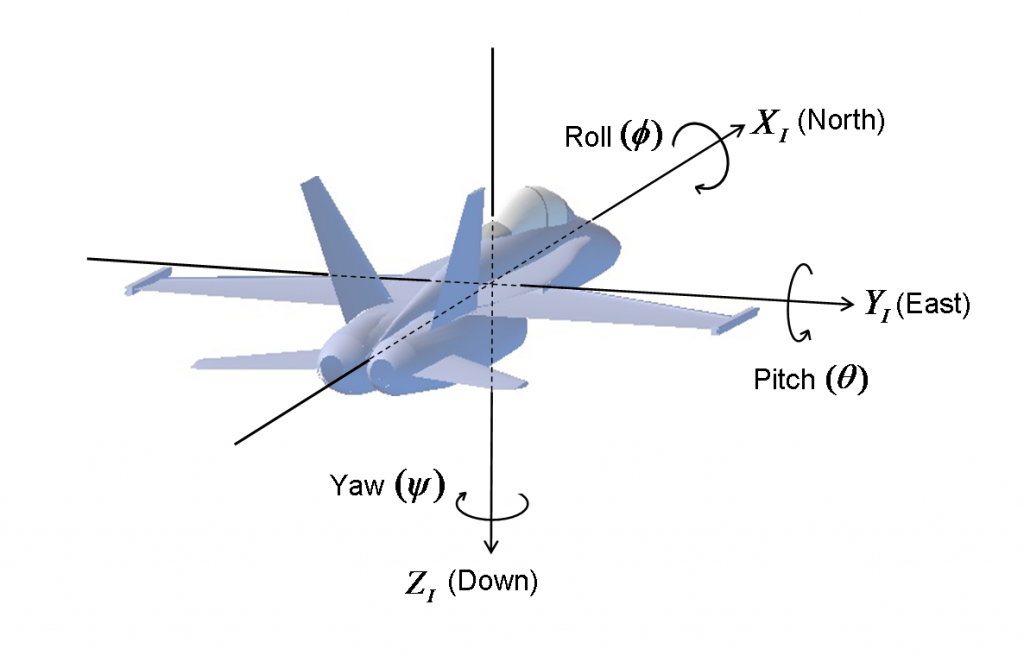
\includegraphics[width=0.6\linewidth]{image_euler_angles} \caption{Euler Angles}\label{fig:unnamed-chunk-4}
\end{figure}

To convert quaternions to euler angles I used \emph{Q2EA} function in
\emph{orientlib} package.(See:
\url{https://www.rdocumentation.org/packages/orientlib/versions/0.10.3})

\begin{Shaded}
\begin{Highlighting}[]
\CommentTok{# define a function to convert quaternion values to euler angles. }
\NormalTok{convert_quaternions_to_euler <-}\StringTok{ }\ControlFlowTok{function}\NormalTok{(a_dataset)\{}
    
    \CommentTok{# use Q2EA from RSpincalc to convert quaternions to euler angles}
\NormalTok{    Q <-}\StringTok{ }\NormalTok{a_dataset }\OperatorTok\StringTok{ }\KeywordTok{select}\NormalTok{(}
\NormalTok{                    orientation_X, }
\NormalTok{                    orientation_Y, }
\NormalTok{                    orientation_Z, }
\NormalTok{                    orientation_W) }\OperatorTok\StringTok{ }
\StringTok{                }\KeywordTok{as.matrix}\NormalTok{()}
    
\NormalTok{    euler_matrix <-}\StringTok{ }\KeywordTok{Q2EA}\NormalTok{(Q, }
                 \DataTypeTok{EulerOrder=}\StringTok{'xyz'}\NormalTok{, }
                 \DataTypeTok{tol =} \DecValTok{10} \OperatorTok{*}\StringTok{ }\NormalTok{.Machine}\OperatorTok{$}\NormalTok{double.eps, }
                 \DataTypeTok{ichk =} \OtherTok{FALSE}\NormalTok{, }
                 \DataTypeTok{ignoreAllChk =} \OtherTok{FALSE}\NormalTok{)}

    \CommentTok{# add the new columns to the dataset}
\NormalTok{    a_dataset <-}\StringTok{ }\NormalTok{a_dataset }\OperatorTok\StringTok{ }\KeywordTok{mutate}\NormalTok{(}
                    \DataTypeTok{phi =}\NormalTok{ euler_matrix[,}\DecValTok{1}\NormalTok{],}
                    \DataTypeTok{theta =}\NormalTok{ euler_matrix[,}\DecValTok{2}\NormalTok{], }
                    \DataTypeTok{psi =}\NormalTok{ euler_matrix[,}\DecValTok{3}\NormalTok{])}
    
    \CommentTok{# remove quaternion columns}
\NormalTok{    a_dataset <-}\StringTok{ }\NormalTok{a_dataset }\OperatorTok\StringTok{ }\KeywordTok{select}\NormalTok{(}
                \OperatorTok{-}\NormalTok{orientation_X, }
                \OperatorTok{-}\NormalTok{orientation_Y,  }
                \OperatorTok{-}\NormalTok{orientation_Z, }
                \OperatorTok{-}\NormalTok{orientation_W)}
    
    \CommentTok{# return the new dataset}
\NormalTok{    a_dataset}
\NormalTok{\}}

\NormalTok{x_train <-}\StringTok{ }\KeywordTok{convert_quaternions_to_euler}\NormalTok{(x_train)}
\NormalTok{x_test <-}\StringTok{ }\KeywordTok{convert_quaternions_to_euler}\NormalTok{(x_test)}
\end{Highlighting}
\end{Shaded}

Distribution of orientation angles by surface:

\includegraphics{PH125_9_CYO_Report_files/figure-latex/unnamed-chunk-5-1.pdf}

It looks like the most noticeable differences between surfaces can be
observed in the orientation distribution.

If we consider unit of time to be 1, we can draw the path of the robot
movement. In the following figures I draw the path for several cases,
faceted by surface. I expect that the surface would influence the shape
of these paths.

\includegraphics{PH125_9_CYO_Report_files/figure-latex/draw path-1.pdf}
\includegraphics{PH125_9_CYO_Report_files/figure-latex/draw path-2.pdf}

\hypertarget{data-pre-processing}{%
\section{Data Pre-Processing}\label{data-pre-processing}}

An important step in fitting a good model is pre-processing the data. In
our case we havee series of observation of 128 measurements. In this
section I will create aggregations around these measurement. These are:
mean, standard deviation, distances of segments from one point to the
next. total distance, total angle change both from magnetostatic and
gyro sensors. All of these are encapsulated in the following function:

\begin{Shaded}
\begin{Highlighting}[]
\CommentTok{# function for pre-processing }
\CommentTok{# n_of_rows defaults to total number ofseries}
\CommentTok{# is_train indicates that the data is training, thus will do an extra action}
\NormalTok{pre_process <-}\StringTok{ }\ControlFlowTok{function}\NormalTok{(a_dataframe, }\DataTypeTok{n_of_rows =} \KeywordTok{nrow}\NormalTok{(a_dataframe)}\OperatorTok{/}\DecValTok{128}\NormalTok{ ) \{}
    
    \CommentTok{# get data grouped by seeries_id and compute some means }
\NormalTok{    processed_data_df <-}\StringTok{ }\NormalTok{a_dataframe }\OperatorTok\StringTok{ }
\StringTok{    }\KeywordTok{group_by}\NormalTok{(series_id) }\OperatorTok\StringTok{ }
\StringTok{    }\KeywordTok{summarize}\NormalTok{(}
        \DataTypeTok{phi_mean_all =} \KeywordTok{mean}\NormalTok{(phi),}
        \DataTypeTok{phi_sd_all =} \KeywordTok{sd}\NormalTok{(phi),}
        \DataTypeTok{phi_mean_to_sd_all =} \KeywordTok{mean}\NormalTok{(phi)}\OperatorTok{/}\KeywordTok{sd}\NormalTok{(phi),}
        \DataTypeTok{theta_mean_all =} \KeywordTok{mean}\NormalTok{(theta),}
        \DataTypeTok{theta_sd_all =} \KeywordTok{sd}\NormalTok{(theta),}
        \DataTypeTok{theta_mean_to_sd_all =} \KeywordTok{mean}\NormalTok{(theta)}\OperatorTok{/}\KeywordTok{sd}\NormalTok{(theta),}
        \DataTypeTok{psi_mean_all =} \KeywordTok{mean}\NormalTok{(psi),}
        \DataTypeTok{psi_sd_all =} \KeywordTok{sd}\NormalTok{(psi),}
        \DataTypeTok{psi_mean_to_sd_all =} \KeywordTok{mean}\NormalTok{(psi)}\OperatorTok{/}\KeywordTok{sd}\NormalTok{(psi),}
        \CommentTok{# this is the rectangular area that surounds the path of linear movement}
        \DataTypeTok{dist_area =}\NormalTok{ (}\KeywordTok{max}\NormalTok{(linear_acceleration_X) }\OperatorTok{-}\StringTok{ }\KeywordTok{min}\NormalTok{(linear_acceleration_X)) }\OperatorTok{*}\StringTok{ }\NormalTok{(}\KeywordTok{max}\NormalTok{(linear_acceleration_Y) }\OperatorTok{-}\StringTok{ }\KeywordTok{min}\NormalTok{(linear_acceleration_Y)) }\OperatorTok{+}\StringTok{ }
\StringTok{            }\NormalTok{(}\KeywordTok{max}\NormalTok{(linear_acceleration_X) }\OperatorTok{-}\StringTok{ }\KeywordTok{min}\NormalTok{(linear_acceleration_X)) }\OperatorTok{*}\StringTok{ }\NormalTok{(}\KeywordTok{max}\NormalTok{(linear_acceleration_Z) }\OperatorTok{-}\StringTok{ }\KeywordTok{min}\NormalTok{(linear_acceleration_Z)) }\OperatorTok{+}\StringTok{ }
\StringTok{            }\NormalTok{(}\KeywordTok{max}\NormalTok{(linear_acceleration_Y) }\OperatorTok{-}\StringTok{ }\KeywordTok{min}\NormalTok{(linear_acceleration_Y)) }\OperatorTok{*}\StringTok{ }\NormalTok{(}\KeywordTok{max}\NormalTok{(linear_acceleration_Z) }\OperatorTok{-}\StringTok{ }\KeywordTok{min}\NormalTok{(linear_acceleration_Z)),}
        \CommentTok{# this is the rectangular area that surounds the path of angular movement}
        \DataTypeTok{omega_area =}\NormalTok{ (}\KeywordTok{max}\NormalTok{(angular_velocity_X) }\OperatorTok{-}\StringTok{ }\KeywordTok{min}\NormalTok{(angular_velocity_X)) }\OperatorTok{*}\StringTok{ }\NormalTok{(}\KeywordTok{max}\NormalTok{(angular_velocity_Y) }\OperatorTok{-}\StringTok{ }\KeywordTok{min}\NormalTok{(angular_velocity_Y)) }\OperatorTok{+}
\StringTok{            }\NormalTok{(}\KeywordTok{max}\NormalTok{(angular_velocity_X) }\OperatorTok{-}\StringTok{ }\KeywordTok{min}\NormalTok{(angular_velocity_X)) }\OperatorTok{*}\StringTok{ }\NormalTok{(}\KeywordTok{max}\NormalTok{(angular_velocity_Z) }\OperatorTok{-}\StringTok{ }\KeywordTok{min}\NormalTok{(angular_velocity_Z)) }\OperatorTok{+}
\StringTok{            }\NormalTok{(}\KeywordTok{max}\NormalTok{(angular_velocity_Y) }\OperatorTok{-}\StringTok{ }\KeywordTok{min}\NormalTok{(angular_velocity_Y)) }\OperatorTok{*}\StringTok{ }\NormalTok{(}\KeywordTok{max}\NormalTok{(angular_velocity_Z) }\OperatorTok{-}\StringTok{ }\KeywordTok{min}\NormalTok{(angular_velocity_Z)),}
        \DataTypeTok{euler_area =}\NormalTok{ (}\KeywordTok{max}\NormalTok{(phi) }\OperatorTok{-}\StringTok{ }\KeywordTok{min}\NormalTok{(phi)) }\OperatorTok{*}\StringTok{ }\NormalTok{(}\KeywordTok{max}\NormalTok{(theta) }\OperatorTok{-}\StringTok{ }\KeywordTok{min}\NormalTok{(theta)) }\OperatorTok{+}\StringTok{ }
\StringTok{            }\NormalTok{(}\KeywordTok{max}\NormalTok{(phi) }\OperatorTok{-}\StringTok{ }\KeywordTok{min}\NormalTok{(phi)) }\OperatorTok{*}\StringTok{ }\NormalTok{(}\KeywordTok{max}\NormalTok{(psi) }\OperatorTok{-}\StringTok{ }\KeywordTok{min}\NormalTok{(psi)) }\OperatorTok{+}\StringTok{ }
\StringTok{            }\NormalTok{(}\KeywordTok{max}\NormalTok{(theta) }\OperatorTok{-}\StringTok{ }\KeywordTok{min}\NormalTok{(theta)) }\OperatorTok{*}\StringTok{ }\NormalTok{(}\KeywordTok{max}\NormalTok{(psi) }\OperatorTok{-}\StringTok{ }\KeywordTok{min}\NormalTok{(psi)),}
        \DataTypeTok{dist_mean_x =} \KeywordTok{mean}\NormalTok{(linear_acceleration_X),}
        \DataTypeTok{dist_mean_y =} \KeywordTok{mean}\NormalTok{(linear_acceleration_Y),}
        \DataTypeTok{dist_mean_z =} \KeywordTok{mean}\NormalTok{(linear_acceleration_Z),}
        \DataTypeTok{omega_mean_x =} \KeywordTok{mean}\NormalTok{(angular_velocity_X),}
        \DataTypeTok{omega_mean_y =} \KeywordTok{mean}\NormalTok{(angular_velocity_Y),}
        \DataTypeTok{omega_mean_Z =} \KeywordTok{mean}\NormalTok{(angular_velocity_Z),}
        \DataTypeTok{dist_sd_x =} \KeywordTok{sd}\NormalTok{(linear_acceleration_X),}
        \DataTypeTok{dist_sd_y =} \KeywordTok{sd}\NormalTok{(linear_acceleration_Y),}
        \DataTypeTok{dist_sd_z =} \KeywordTok{sd}\NormalTok{(linear_acceleration_Z),}
        \DataTypeTok{omega_sd_x =} \KeywordTok{sd}\NormalTok{(angular_velocity_X),}
        \DataTypeTok{omega_sd_y =} \KeywordTok{sd}\NormalTok{(angular_velocity_Y),}
        \DataTypeTok{omega_sd_Z =} \KeywordTok{sd}\NormalTok{(angular_velocity_Z) }
        
\NormalTok{        ) }\OperatorTok\StringTok{ }
\StringTok{        }\KeywordTok{slice}\NormalTok{(}\DecValTok{1}\OperatorTok{:}\NormalTok{n_of_rows)}
    
    \CommentTok{# define an empty data frame with summary metrics that we'll use for each set of 128 observations}
\NormalTok{    metrics <-}\StringTok{ }\KeywordTok{c}\NormalTok{(}\StringTok{"dist_total"}\NormalTok{,}\StringTok{"dist_max"}\NormalTok{,}\StringTok{"dist_min"}\NormalTok{,}\StringTok{"dist_max_to_min"}\NormalTok{,}\StringTok{"dist_mean"}\NormalTok{,}\StringTok{"dist_sd"}\NormalTok{,}\StringTok{"dist_mean_to_sd"}\NormalTok{,}
                             \StringTok{"omega_total"}\NormalTok{,}\StringTok{"omega_max"}\NormalTok{,}\StringTok{"omega_min"}\NormalTok{,}\StringTok{"omega_max_to_min"}\NormalTok{,}\StringTok{"omega_mean"}\NormalTok{,}\StringTok{"omega_sd"}\NormalTok{,}\StringTok{"omega_mean_to_sd"}\NormalTok{,}
                             \StringTok{"phi_total"}\NormalTok{,}\StringTok{"phi_max"}\NormalTok{,}\StringTok{"phi_min"}\NormalTok{,}\StringTok{"phi_mean"}\NormalTok{,}\StringTok{"phi_sd"}\NormalTok{,}\StringTok{"phi_mean_to_sd"}\NormalTok{,}
                             \StringTok{"theta_total"}\NormalTok{,}\StringTok{"theta_max"}\NormalTok{,}\StringTok{"theta_min"}\NormalTok{,}\StringTok{"theta_mean"}\NormalTok{,}\StringTok{"theta_sd"}\NormalTok{,}\StringTok{"theta_mean_to_sd"}\NormalTok{,}
                             \StringTok{"psi_total"}\NormalTok{,}\StringTok{"psi_max"}\NormalTok{,}\StringTok{"psi_min"}\NormalTok{,}\StringTok{"psi_mean"}\NormalTok{,}\StringTok{"psi_sd"}\NormalTok{,}\StringTok{"psi_mean_to_sd"}\NormalTok{,}
                             \StringTok{"euler_total"}\NormalTok{,}\StringTok{"euler_max"}\NormalTok{,}\StringTok{"euler_min"}\NormalTok{,}\StringTok{"euler_mean"}\NormalTok{,}\StringTok{"euler_sd"}\NormalTok{,}\StringTok{"euler_mean_to_sd"}\NormalTok{)}
\NormalTok{    tmp_df <-}\StringTok{ }\KeywordTok{data.frame}\NormalTok{(}\KeywordTok{matrix}\NormalTok{(}\DataTypeTok{ncol =} \KeywordTok{length}\NormalTok{(metrics), }\DataTypeTok{nrow =} \DecValTok{0}\NormalTok{) )}
    \KeywordTok{colnames}\NormalTok{(tmp_df) <-}\StringTok{ }\NormalTok{metrics}

    \CommentTok{# loop over each series and compute aggegations}
    \CommentTok{# should use apply type of function here, but I use "for" until I master the apply}
    \ControlFlowTok{for}\NormalTok{ (s_id }\ControlFlowTok{in}\NormalTok{ processed_data_df}\OperatorTok{$}\NormalTok{series_id)}
\NormalTok{    \{}
        \CommentTok{# get current measurement set}
\NormalTok{        this_chunk_df <-}\StringTok{ }\NormalTok{a_dataframe }\OperatorTok\StringTok{ }\KeywordTok{filter}\NormalTok{(series_id }\OperatorTok{==}\StringTok{ }\NormalTok{s_id)}
        
        \CommentTok{# select only columns we are interested in }
\NormalTok{        this_chunk_df <-}\StringTok{ }\NormalTok{this_chunk_df }\OperatorTok\StringTok{ }
\StringTok{            }\KeywordTok{select}\NormalTok{(}
\NormalTok{            phi, theta, psi,  }
\NormalTok{            angular_velocity_X, angular_velocity_Y, angular_velocity_Z,}
\NormalTok{            linear_acceleration_X, linear_acceleration_Y, linear_acceleration_Z)}
        \CommentTok{# this is a vector with euclidian distances from one point to the next}
\NormalTok{        dist_v <-}\StringTok{ }\KeywordTok{sqrt}\NormalTok{(}\KeywordTok{diff}\NormalTok{(this_chunk_df}\OperatorTok{$}\NormalTok{linear_acceleration_X)}\OperatorTok{^}\DecValTok{2} \OperatorTok{+}\StringTok{ }\KeywordTok{diff}\NormalTok{(this_chunk_df}\OperatorTok{$}\NormalTok{linear_acceleration_Y)}\OperatorTok{^}\DecValTok{2} \OperatorTok{+}\StringTok{ }\KeywordTok{diff}\NormalTok{(this_chunk_df}\OperatorTok{$}\NormalTok{linear_acceleration_Z)}\OperatorTok{^}\DecValTok{2}\NormalTok{)}
\NormalTok{        omega_v <-}\StringTok{ }\KeywordTok{sqrt}\NormalTok{(}\KeywordTok{diff}\NormalTok{(this_chunk_df}\OperatorTok{$}\NormalTok{angular_velocity_X)}\OperatorTok{^}\DecValTok{2} \OperatorTok{+}\StringTok{ }\KeywordTok{diff}\NormalTok{(this_chunk_df}\OperatorTok{$}\NormalTok{angular_velocity_Y)}\OperatorTok{^}\DecValTok{2} \OperatorTok{+}\StringTok{ }\KeywordTok{diff}\NormalTok{(this_chunk_df}\OperatorTok{$}\NormalTok{angular_velocity_Z)}\OperatorTok{^}\DecValTok{2}\NormalTok{)}
\NormalTok{        phi_v <-}\StringTok{ }\KeywordTok{abs}\NormalTok{(}\KeywordTok{diff}\NormalTok{(this_chunk_df}\OperatorTok{$}\NormalTok{phi))}
\NormalTok{        theta_v <-}\StringTok{ }\KeywordTok{abs}\NormalTok{(}\KeywordTok{diff}\NormalTok{(this_chunk_df}\OperatorTok{$}\NormalTok{theta))}
\NormalTok{        psi_v <-}\StringTok{ }\KeywordTok{abs}\NormalTok{(}\KeywordTok{diff}\NormalTok{(this_chunk_df}\OperatorTok{$}\NormalTok{psi))}

        \CommentTok{# fill or temp data frame with summary computations for our 128 measurement set}
\NormalTok{        tmp_df <-}\StringTok{ }\KeywordTok{bind_rows}\NormalTok{(tmp_df, }\KeywordTok{data_frame}\NormalTok{(}
            
            \CommentTok{# all features starting with "dist_" refers to linear movement}
            \DataTypeTok{dist_total =} \KeywordTok{sum}\NormalTok{(dist_v),}
            \DataTypeTok{dist_max =} \KeywordTok{max}\NormalTok{(dist_v),}
            \DataTypeTok{dist_min =} \KeywordTok{min}\NormalTok{(dist_v),}
            \DataTypeTok{dist_max_to_min =} \KeywordTok{max}\NormalTok{(dist_v)}\OperatorTok{/}\KeywordTok{min}\NormalTok{(dist_v),}
            \DataTypeTok{dist_mean =} \KeywordTok{mean}\NormalTok{(dist_v),}
            \DataTypeTok{dist_sd =} \KeywordTok{sd}\NormalTok{(dist_v),}
            \DataTypeTok{dist_mean_to_sd =} \KeywordTok{mean}\NormalTok{(dist_v)}\OperatorTok{/}\KeywordTok{sd}\NormalTok{(dist_v),  }\CommentTok{# reciprocal coef of variation}
            
            \CommentTok{# all features starting with "omega_" refers to angle velocity measurments}
            \DataTypeTok{omega_total =} \KeywordTok{sum}\NormalTok{(omega_v),}
            \DataTypeTok{omega_max =} \KeywordTok{max}\NormalTok{(omega_v),}
            \DataTypeTok{omega_min =} \KeywordTok{min}\NormalTok{(omega_v),}
            \DataTypeTok{omega_max_to_min =} \KeywordTok{max}\NormalTok{(omega_v)}\OperatorTok{/}\KeywordTok{min}\NormalTok{(omega_v),}
            \DataTypeTok{omega_mean =} \KeywordTok{mean}\NormalTok{(omega_v),}
            \DataTypeTok{omega_sd =} \KeywordTok{sd}\NormalTok{(omega_v),}
            \DataTypeTok{omega_mean_to_sd =} \KeywordTok{mean}\NormalTok{(omega_v)}\OperatorTok{/}\KeywordTok{sd}\NormalTok{(omega_v), }\CommentTok{# reciprocal coef of variation}

            \CommentTok{# phi, theta and psi reffers to roll, pitch and yaw rotations}
            \DataTypeTok{phi_total =} \KeywordTok{sum}\NormalTok{(phi_v),}
            \DataTypeTok{phi_max =} \KeywordTok{max}\NormalTok{(phi_v),}
            \DataTypeTok{phi_min =} \KeywordTok{min}\NormalTok{(phi_v),}
            \DataTypeTok{phi_mean =} \KeywordTok{mean}\NormalTok{(phi_v),}
            \DataTypeTok{phi_sd =} \KeywordTok{sd}\NormalTok{(phi_v),}
            \DataTypeTok{phi_mean_to_sd =} \KeywordTok{mean}\NormalTok{(phi_v)}\OperatorTok{/}\KeywordTok{sd}\NormalTok{(phi_v),}
            
            \DataTypeTok{theta_total =} \KeywordTok{sum}\NormalTok{(theta_v),}
            \DataTypeTok{theta_max =} \KeywordTok{max}\NormalTok{(theta_v),}
            \DataTypeTok{theta_min =} \KeywordTok{min}\NormalTok{(theta_v),}
            \DataTypeTok{theta_mean =} \KeywordTok{mean}\NormalTok{(theta_v),}
            \DataTypeTok{theta_sd =} \KeywordTok{sd}\NormalTok{(theta_v),}
            \DataTypeTok{theta_mean_to_sd =} \KeywordTok{mean}\NormalTok{(theta_v)}\OperatorTok{/}\KeywordTok{sd}\NormalTok{(theta_v),}
            
            \DataTypeTok{psi_total =} \KeywordTok{sum}\NormalTok{(psi_v),}
            \DataTypeTok{psi_max =} \KeywordTok{max}\NormalTok{(psi_v),}
            \DataTypeTok{psi_min =} \KeywordTok{min}\NormalTok{(psi_v),}
            \DataTypeTok{psi_mean =} \KeywordTok{mean}\NormalTok{(psi_v),}
            \DataTypeTok{psi_sd =} \KeywordTok{sd}\NormalTok{(psi_v),}
            \DataTypeTok{psi_mean_to_sd =} \KeywordTok{mean}\NormalTok{(psi_v)}\OperatorTok{/}\KeywordTok{sd}\NormalTok{(psi_v),}
            
            \CommentTok{# features starting with "euler_" refers to }
            \CommentTok{# agragation of all phi, theta and psi rotations}
            \DataTypeTok{euler_total =} \KeywordTok{sum}\NormalTok{(phi_v }\OperatorTok{+}\StringTok{ }\NormalTok{theta_v }\OperatorTok{+}\StringTok{ }\NormalTok{psi_v), }
            \DataTypeTok{euler_max =} \KeywordTok{max}\NormalTok{(phi_v }\OperatorTok{+}\StringTok{ }\NormalTok{theta_v }\OperatorTok{+}\StringTok{ }\NormalTok{psi_v),}
            \DataTypeTok{euler_min =} \KeywordTok{min}\NormalTok{(phi_v }\OperatorTok{+}\StringTok{ }\NormalTok{theta_v }\OperatorTok{+}\StringTok{ }\NormalTok{psi_v),}
            \DataTypeTok{euler_mean =} \KeywordTok{mean}\NormalTok{(phi_v }\OperatorTok{+}\StringTok{ }\NormalTok{theta_v }\OperatorTok{+}\StringTok{ }\NormalTok{psi_v),}
            \DataTypeTok{euler_sd =} \KeywordTok{sd}\NormalTok{(phi_v }\OperatorTok{+}\StringTok{ }\NormalTok{theta_v }\OperatorTok{+}\StringTok{ }\NormalTok{psi_v),}
            \DataTypeTok{euler_mean_to_sd =} \KeywordTok{mean}\NormalTok{(phi_v }\OperatorTok{+}\StringTok{ }\NormalTok{theta_v }\OperatorTok{+}\StringTok{ }\NormalTok{psi_v)}\OperatorTok{/}\KeywordTok{sd}\NormalTok{(phi_v }\OperatorTok{+}\StringTok{ }\NormalTok{theta_v }\OperatorTok{+}\StringTok{ }\NormalTok{psi_v)}
\NormalTok{            ))}
    
\NormalTok{    \} }\CommentTok{# end of for over series}
    
    \CommentTok{# add the summary computations to the data set of series}
\NormalTok{    processed_data_df <-}\StringTok{ }\KeywordTok{bind_cols}\NormalTok{(processed_data_df, tmp_df)}

    \CommentTok{# more features}
    \CommentTok{# I added thesee as an experimentation after observing the dependencies graphs}
    \CommentTok{# will explain later}
\NormalTok{    processed_data_df <-}\StringTok{ }\NormalTok{processed_data_df }\OperatorTok\StringTok{ }\KeywordTok{mutate}\NormalTok{(}
        \CommentTok{# this is an agular momentum }
        \DataTypeTok{f1 =} \KeywordTok{log}\NormalTok{(dist_mean_to_sd}\OperatorTok{*}\NormalTok{omega_mean_to_sd),}
        
        \CommentTok{# this is an angular momentum }
        \DataTypeTok{f2 =} \KeywordTok{log}\NormalTok{(dist_total}\OperatorTok{*}\NormalTok{omega_total),}
        
        \CommentTok{# this is the angle between theta and psi vectors}
        \DataTypeTok{f3 =} \KeywordTok{abs}\NormalTok{(}\KeywordTok{atan}\NormalTok{(theta_mean_all}\OperatorTok{/}\NormalTok{psi_mean_all)))        }
    
    \CommentTok{# return the proceessed data}
\NormalTok{    processed_data_df}
\NormalTok{\}}
\end{Highlighting}
\end{Shaded}

\hypertarget{more-data-analysis}{%
\subsection{More Data Analysis}\label{more-data-analysis}}

\hypertarget{fit-the-model}{%
\section{Fit The Model}\label{fit-the-model}}

\hypertarget{one-vs-one-or-one-vs-all}{%
\subsection{One-vs-One or One-vs-All}\label{one-vs-one-or-one-vs-all}}

\hypertarget{results-and-submit-the-data}{%
\section{Results and Submit the
Data}\label{results-and-submit-the-data}}

\hypertarget{conclusion}{%
\section{Conclusion}\label{conclusion}}

One of the most important outcome of this prroject is that I learned a
few things in addition to what was presented in the course.

\hypertarget{reference}{%
\section{Reference}\label{reference}}

\begin{enumerate}
\def\labelenumi{\arabic{enumi}.}
\item
  Applied Predictive Modeling - Max Kuhn, Kjell Johnson
\item
  Q2EA: Convert from rotation Quaternions to Euler Angles. Q2EA converts
  from Quaternions (Q) to Euler Angles (EA) based on D. M. Henderson
  (1977). Q2EA.Xiao is the algorithm by J. Xiao (2013) for the Princeton
  Vision Toolkit. \url{https://rdrr.io/cran/RSpincalc/man/Q2EA.html}
\item
  Understanding Quaternions.
  \url{http://www.chrobotics.com/library/understanding-quaternions}
\item
  Understanding Euler Angles.
  \url{http://www.chrobotics.com/library/understanding-euler-angles}
\item
  Tune Machine Learning Algorithms in R (random forest case study) by
  Jason Brownlee.
  \url{https://machinelearningmastery.com/tune-machine-learning-algorithms-in-r/}
\item
  Classification with more than two classes, from Introduction to
  Information Retrieval, Christopher D. Manning, Prabhakar Raghavan and
  Hinrich Schütze,, Cambridge University Press 2008
  \url{https://nlp.stanford.edu/IR-book/html/htmledition/classification-with-more-than-two-classes-1.html}
\item
  A Guide To using IMU (Accelerometer and Gyroscope Devices) in Embedded
  Applications - \url{http://www.starlino.com/imu_guide.html}
\end{enumerate}


\end{document}
